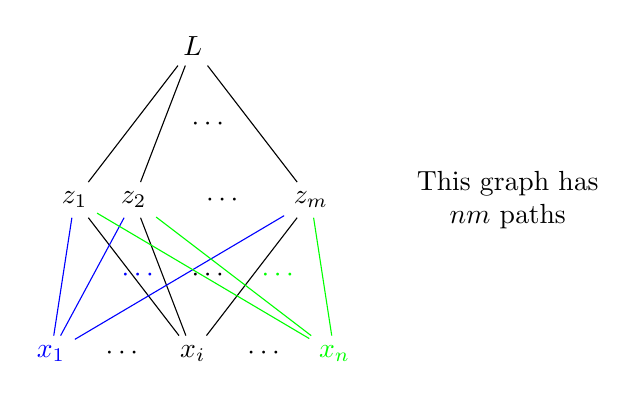
\begin{tikzpicture}
	\begin{scope}[scale=1.5,yscale=1.3]
		\node (L) at (0,1) {$L$};
	 	\node (z1) at (-1,0) {$z_1$};
	 	\node (z2) at (-0.5,0) {$z_2$};
	 	\node (zdots) at (0.25,0) {$\cdots$};
	 	\node (zm) at (1,0) {$z_m$};
	 	\node (xi) at (0,-1) {$x_i$};
	 	
	 	\node[blue] (x1) at (-1.2,-1) {$x_1$};
	 	\node (xdots1) at (-0.6,-1) {$\cdots $};
	 	\node (xdots1) at (0.6,-1) {$\cdots $};
	 	\node[green] (xn) at (1.2,-1) {$x_n$};
 	\end{scope}
 	
 	\path[-] (L) edge node {} (z1);
 	\path[-] (L) edge node {} (z2);
 	\path (L) -- node {$\cdots$} (zdots);
 	\path[-] (L) edge node {} (zm);
 	\path[-] (z1) edge node {} (xi);
 	\path[-] (z2) edge node {} (xi);
 	\path[-] (zdots) -- node {$\cdots$} (xi);
 	\path[-] (zm) edge node {} (xi);

 	\path[-,blue] (z1) edge node {} (x1);
 	\path[-,blue] (z2) edge node {} (x1);
 	\path[-,blue] (zdots) -- node {$\cdots$} (x1);
 	\path[-,blue] (zm) edge node {} (x1);

 	\path[-,green] (z1) edge node {} (xn);
 	\path[-,green] (z2) edge node {} (xn);
 	\path[-,green] (zdots) -- node {$\cdots$} (xn);
 	\path[-,green] (zm) edge node {} (xn);

\node[align=center] at (4,0) {This graph has\\$nm$ paths};
\end{tikzpicture}
